\section{Methodology}
\label{sec:methodology}

\subsection{Primary Dataset and Split}

The primary experiments used the 25,331-image ISIC 2019 training release. The
aggregate collection includes images originating from HAM10000, BCN20000, and
MSK sources
\cite{tschandl2018ham10000,combalia2019bcn20000,codella2017isic}.

The original labels were mapped as follows:
NV, BKL, DF, and VASC formed the non-malignant class; MEL mapped to melanoma;
BCC mapped to BCC; and SCC mapped to SCC. Actinic keratosis was excluded
rather than forced into a malignant or non-malignant endpoint. Four images
belonging to label-conflicting duplicate components were also excluded,
leaving 24,460 eligible four-class images.

Images connected by a shared non-empty lesion identifier or identical
SHA-256 image hash were joined into split groups and assigned intact to the
training, validation, or internal-test partition using a diagnosis-stratified
70/15/15 procedure with seed 42. The audit found no cross-partition overlap in
split-group identifiers, available lesion identifiers, or exact hashes.
However, patient identifiers were unavailable and 2,084 images lacked lesion
identifiers. The procedure is therefore described as leakage-aware or
known-relation-disjoint, not fully patient-independent.

\begin{table}[t]
    \centering
    \caption{Primary four-class dataset distribution.}
    \label{tab:data_distribution}
    \footnotesize
    \setlength{\tabcolsep}{4.1pt}
    \begin{tabular}{lrrr}
        \toprule
        Class & Train & Validation & Test \\
        \midrule
        Non-malignant & 11,193 & 2,398 & 2,398 \\
        Melanoma      &  3,164 &   678 &   678 \\
        BCC           &  2,327 &   498 &   498 \\
        SCC           &    440 &    94 &    94 \\
        \midrule
        Total         & 17,124 & 3,668 & 3,668 \\
        \bottomrule
    \end{tabular}
\end{table}

All principal models were evaluated on the same locked 3,668-image test
partition.

\subsection{Preprocessing}

All models used $224\times224$ RGB inputs and ImageNet normalisation.
Training transformations consisted of random resized cropping with scale
$0.85$--$1.00$ and aspect ratio $0.90$--$1.10$, horizontal and vertical
flips with probability 0.5, rotation within $\pm15^{\circ}$, and mild colour
jitter. Validation and test preprocessing deterministically resized the
shorter side to 256 pixels and applied a $224\times224$ centre crop. No
stochastic validation or test augmentation was used.

\subsection{Models and Conditional Inference}

Figure~\ref{fig:architecture} illustrates the backbone-matched EfficientNet-B0
comparison.

\begin{figure*}[t]
    \centering
    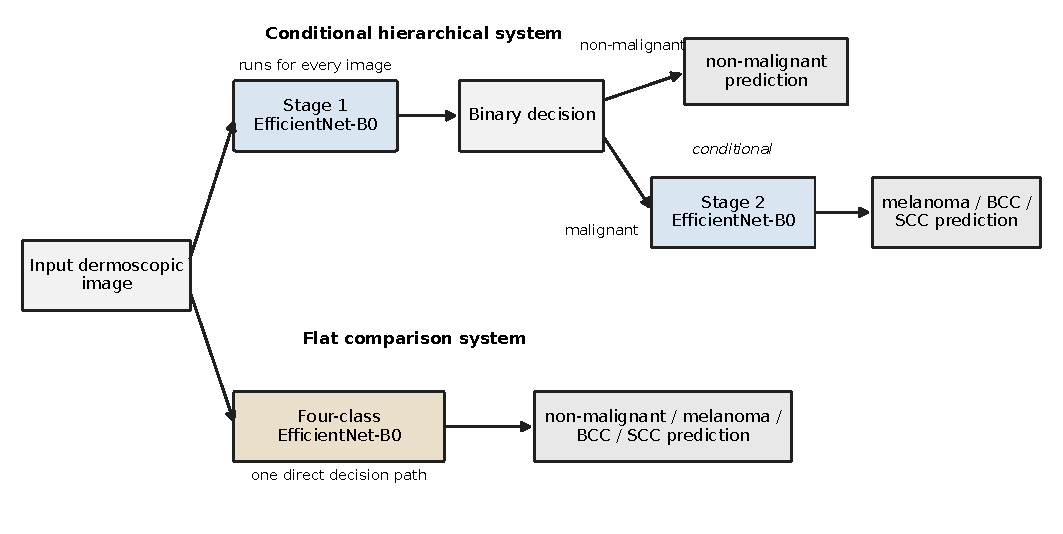
\includegraphics[width=0.96\textwidth]
    {figures/figure01_architecture.pdf}
    \caption{Backbone-matched EfficientNet-B0 comparison. The flat system directly
    predicts one of four classes. The hierarchy first predicts
    non-malignant versus malignant and invokes Stage~2 only for predicted
    malignant images. The DenseNet-121 flat comparator and standalone
    T-category experiment are not shown.}
    \label{fig:architecture}
\end{figure*}

The flat EfficientNet-B0 model used an ImageNet-initialised backbone with a
four-output classifier and ordinary cross-entropy. The flat DenseNet-121 model
used the same split, transformations, cross-entropy protocol, optimiser,
scheduler, validation-selection metric, seed, and locked-test policy; only the
backbone implementation changed.

The hierarchy used two independently trained ImageNet-initialised
EfficientNet-B0 models. Stage~1 had two outputs and used ordinary
cross-entropy. Stage~2 had three outputs ordered as melanoma, BCC, and SCC.
Cross-entropy, inverse-frequency weighted cross-entropy, and class-balanced
focal loss were compared using validation macro-F1. The selected Stage~2
model used class-balanced focal loss with effective-number parameter
$\beta=0.9999$ and focal parameter $\gamma=2.0$:
\begin{equation}
\mathcal{L}_{\mathrm{CBF}}
=
-w_y(1-p_y)^{\gamma}\log p_y.
\end{equation}

At inference, Stage~1 ran for every image. An argmax non-malignant prediction
terminated the path, while an argmax malignant prediction invoked Stage~2.
No internal-test threshold tuning was performed.

\subsection{Training Protocol}

Full runs used batch size 64, at most 30 epochs, and automatic mixed precision
on an NVIDIA Tesla T4. AdamW used learning rate $3\times10^{-4}$ and weight
decay $10^{-4}$. Cosine annealing reduced the learning rate toward
$10^{-6}$. All experiments used seed 42, early-stopping patience seven, and
validation macro-F1 for checkpoint selection. The internal test was not used
for loss, threshold, hyperparameter, or checkpoint selection.

The frozen checkpoints corresponded to epoch 2 for flat EfficientNet-B0,
epoch 4 for flat DenseNet-121, epoch 5 for Stage~1, and epoch 8 for the
selected Stage~2 model.

\subsection{Standalone T-Category Experiment}

A candidate identifier list was used only to locate public ISIC records. No
images from that external repository or the Dermoscopy Atlas were used.
Official ISIC Archive metadata supplied authoritative labels, licensing, and
attribution.

Of 856 candidates, 848 were eligible. Broad labels were derived from official
diagnosis and Breslow-thickness metadata: in situ as Tis,
$0$--$1$\,mm as T1, $>1$--$2$\,mm as T2,
$>2$--$4$\,mm as T3, and $>4$\,mm as T4. The leakage-aware split contained
594 training, 127 validation, and 127 test images. Training counts were
355, 184, 33, 10, and 12 for Tis through T4. The selected
EfficientNet-B0 model used inverse-frequency weighted cross-entropy and the
epoch-12 validation-selected checkpoint.

\subsection{Evaluation and Statistical Protocol}

Accuracy, balanced accuracy, macro-F1, weighted-F1, per-class metrics, and
confusion matrices were reported. For all pairwise model comparisons, predictions were aligned by image
identifier and analysed using 10,000 ground-truth-class-stratified paired
bootstrap replicates with seed 42 and percentile 95\% confidence intervals.
Exact two-sided McNemar tests were used to assess differences in paired
correctness.
